% Template for PLoS
% Version 1.0 January 2009

\documentclass[10pt]{article}

% amsmath package, useful for mathematical formulas
\usepackage{amsmath}
% amssymb package, useful for mathematical symbols
\usepackage{amssymb}

% graphicx package, useful for including eps and pdf graphics
% include graphics with the command \includegraphics
\usepackage{graphicx}

% cite package, to clean up citations in the main text. Do not remove.
\usepackage{cite}

\usepackage{color} 

% Use doublespacing - comment out for single spacing
%\usepackage{setspace} 
%\doublespacing


% Text layout
\topmargin 0.0cm
\oddsidemargin 0.5cm
\evensidemargin 0.5cm
\textwidth 16cm 
\textheight 21cm

% Bold the 'Figure #' in the caption and separate it with a period
% Captions will be left justified
\usepackage[labelfont=bf,labelsep=period,justification=raggedright]{caption}

% Use the PLoS provided bibtex style
\bibliographystyle{plos2009}

% Remove brackets from numbering in List of References
\makeatletter
\renewcommand{\@biblabel}[1]{\quad#1.}
\makeatother


% Leave date blank
\date{}

\pagestyle{myheadings}
%% ** EDIT HERE **


%% ** EDIT HERE **
%% PLEASE INCLUDE ALL MACROS BELOW

\newcommand{\Kcomment}[1]{{\color{blue}{[KJ: #1]}}}
\newcommand{\Acomment}[1]{{\color{red}{[AE: #1]}}}

\DeclareMathOperator{\Tr}{tr}
\newcommand{\mcond}{\,\middle\vert\,}
\newcommand{\cond}{\,\vert\,}
\newcommand{\loss}[1]{\mathcal L\left(#1\right)} 
\newcommand{\T}{{\sf T}}
\newcommand{\E}[2][]{\mathbb E_{#1}\left[ #2\right]}    % expected value
\newcommand{\TODO}[1]{\emph{\small\color{blue}$\langle\langle$#1$\rangle\rangle$}}
\newcommand*\dif{\mathop{}\,d}
\DeclareMathOperator*{\argmin}{arg\,min}
\DeclareMathOperator{\rank}{rank}

%% END MACROS SECTION

\begin{document}
% Title must be 150 characters or less
\begin{flushleft}
{\Large
Improved estimation of neural correlations suggests detailed interactions in visual cortex
}
% Insert Author names, affiliations and corresponding author email.
\\
Dimitri Yatsenko,$^{1,\ast}$, 
Kre\v{s}imir Josi\'{c}$^{2}$,
Alexander S.~Ecker$^{1,3,4}$,
Emmanouil Froudarakis$^{1}$,
R.~James Cotton$^{1}$,
Andreas S.~Tolias$^{1,5}$
\\
\bf{1} Department of Neuroscience, Baylor College of Medicine, Houston, TX, USA
\\
\bf{2} Department of Mathematics and Department of Biology and Biochemistry, University of Houston, Houston, TX, USA
\\
\bf{3}  Werner Reichardt Center for Integrative Neuroscience and Institute for Theoretical Physics, University of T\"ubingen, Germany
\\
\bf{4} Bernstein Center for Computational Neuroscience, T\"ubingen, Germany
\\
\bf{5} Department of Computational and Applied Mathematics, Rice University, Houston, TX, USA

$\ast$ E-mail: yatsenko@cns.bcm.edu
\end{flushleft}

\section*{Abstract}
% Please keep the abstract between 250 and 300 words
Ambitious projects currently under way aim to record the activity of ever larger and denser subsets of neurons in behaving animals.  It is anticipated that correlations measured in such recordings will uncover aspects of functional organization of neural circuits.  However, estimation and interpretation of large correlation matrices from finite recordings can be challenging.  Estimation can be improved by regularization: the biasing of the estimate toward a low-dimensional, less variable approximation.  The amount of improvement depends on how closely the reduced approximation captures the dominant interactions with fewest terms.  Therefore, the selection of the most efficient estimator is an empirical question dependent on the system under investigation.

We compared regularized correlation matrix estimators biased toward four respective families of low-dimensional correlation structures: independent, latent factors, sparse partial correlations, and sparse partial correlations with latent factors.  The estimators' performance was evaluated on the noise correlation matrices from spatially compact groups of 91--314 neurons (average 206) in mouse visual cortex (31 sites in 24 animals) acquired by \emph{in vivo} fast 3D random-access two-photon imaging of calcium signals.  Recordings lasting between 15 and 20 minutes were deconvolved and binned at 150 ms.  Each estimator was optimized and evaluated by nested cross-validation.  We found that both sparse partial correlations and latent factors were required for efficient estimation.  In addition to reducing estimation error, optimized estimates provided compact representations of the correlation structure consisting of a sparse network of pairwise interactions and global diffuse fluctuations.  The density of positive interactions in these networks decreased rapidly with distance and with difference in orientation preference, whereas negative interactions were less selective.  The physiological interpretation of these components remains in question and must be addressed by future experiments where synaptic connectivity, cell types, and local field potentials may be used to corroborate such interpretations.

\section*{Author Summary}
% Please keep the Author Summary between 150 and 200 words
% Use first person. PLoS ONE authors please skip this step. 
% Author Summary not valid for PLoS ONE submissions.   
Correlation matrices of the activity of populations of neurons are useful descriptors of their functional organization with implications for stimulus coding and circuit architecture.  Estimates of the correlation matrix can be dramatically improved by \emph{regularization}: the biasing of the estimate toward one of several possible low-dimensional approximations.  Using synthetic data, we demonstrated that different estimators performed better or worse than others depending on how well their regularization targets captured the structure of the true correlation matrix.  Then, we compared the performance of several estimators on the population calcium activity of relatively large and dense groups of neurons in mouse visual cortex under visual stimulation.  We found that the best estimator for such neural data was composed of a sparse network of partial correlations between pairs of neurons combined with several latent units interacting with the entire population. We hypothesize that such succinct representations of the correlation structure may more accurately reflect the circuit's functional organization than the conventional correlations.  
\section*{Introduction}
Pearson correlations between the spiking activity of pairs of neurons, or simply \emph{neural correlations}, are the most familiar descriptive statistics of neural population activity \cite{Averbeck:2006,Zohary:1994,Kohn:2005,Bair:2001,Renart:2010}.  For example, \emph{noise correlations}, \emph{i.e.}~the correlations of stimulus response variability between pairs of neurons, have been shown to have profound theoretical implications for stimulus coding \cite{Zohary:1994,Abbott:1999,Averbeck:2006,Berens:2011,Ecker:2011}. In addition, neural correlations are hypothesized to reflect aspects of functional connectivity in neural circuits.  Such interpretation is supported by a series of discoveries of nontrivial relationships between neural correlations and other aspects of circuit organization such as the physical distance separating the neurons \cite{Smith:2008,Denman:2013}, their synaptic connectivity \cite{Ko:2011},  stimulus tuning similarity \cite{Kohn:2005,Ko:2011}, cortical layer specificity \cite{Hansen:2012,Smith:2013}, progressive changes in development and in learning \cite{Golshani:2009}, changes due to sensory stimulation and global brain states \cite{Goard:2009,Kohn:2009,Ecker:2010,Renart:2010}, and others.

However, neural correlations do not submit to ready or unambiguous mechanistic interpretation.  Theoretical studies and simulations have shown that neural correlations on various temporal scales may arise from combinations of multiple mechanisms including  direct synaptic interactions, common inputs or correlated inputs, chains of multiple synaptic connections, oscillations, top-down modulation, and background network fluctuations \cite{Perkel:1967b,Shadlen:1998,Salinas:2001,Ostojic:2009,Rosenbaum:2011}.

A correlation matrix provides more information than the equivalent number of pairwise correlations assessed in isolation.  Yet early studies of neural correlations were based on measurements from isolated pairs of neurons; the effects of correlations on neural coding were then extrapolated in simulations and theoretical studies \cite{Shadlen:1998,Zohary:1994}.  Modern multineuronal recordings from increasingly large and dense subsets of neurons in intact circuits allow estimating the entire correlation matrix of large populations of highly interconnected neurons.  Such estimates can be transformed into various representations that express different aspects of the correlation structure and may suggest different mechanistic interpretations.  For example, factor analysis or principle component analysis may reveal common activity fluctuations across the entire population \cite{Yu:2009}.  The correlation matrix also allows computing the \emph{partial correlations} between specific pairs of neurons, \emph{i.e.}\;correlations that remain after accounting for the linear effects of all other recorded cells.  Under several assumptions (predominance of linear effects ( sufficiently complete sampling of interacting neurons, and sufficient sample size), partial correlations may better reflect the direct statistical associations or interactions between pairs of neurons. In multivariate normal distributions, zero partial correlations between pairs of variables indicate conditional independence or lack of interaction between the pair and the network of non-zero interactions constitute Gaussian Graphical Models or Gauss-Markov Random Fields \cite{Koller:2009}. With other distributions, the correspondence between conditional dependence and partial correlations diminishes or breaks down \cite{Loh:2012}. Estimation of networks of partial correlations (sometimes called \emph{association networks}) have been applied to map gene interactions \cite{Schafer:2005,Peng:2009} or to establish functional connectivity between brain regions from fMRI data \cite{Varoquaux:2012,Ryali:2012}. 

Multineuronal recordings also present major challenges for the estimation and interpretation of correlations.  As the population size increases, the amount of recorded data grows only linearly whereas the number of estimated coefficients grows quadratically.  This mismatch leads to increased opportunities for spurious correlations, overestimation of shared activity (\emph{i.e.}\;overestimation of large eigenvalues) \cite{Ledoit:2004}, and poorly conditioned estimates of the partial correlations \cite{Schafer:2005}.

In this study, we pursued two related aims: (a)~improved estimation of neural correlation matrices and (b)~discovery of low-dimensional structure of correlations in recordings of multineuronal activity to facilitate their interpretation.

Estimation of the correlation matrix relies on estimating the means and variances of the activity of individual cells.  To estimate the mean activity, we resort to the usual \emph{sample mean} without attempting to improve it. An estimate of the \emph{covariance matrix}  combined estimate of the variances and correlations constitutes an estimate covariance matrix. The problem can then be formulated as finding the optimal estimation of the covariance matrix given the estimate of the mean firing rates.

Estimation can be improved through \emph{regularization}: the deliberate biasing of the estimate toward one of several possible low-dimensional approximations called here \emph{target estimates} \cite{Schafer:2005,Bickel:2006}.  The usual estimate, the \emph{sample covariance matrix} has the advantage of being unbiased but, on average, it falls far from the true covariance matrix because of its sensitivity to sampling noise in the data.  Low-dimensional estimates of various forms are less susceptible to sampling noise but are also liable to introduce their respective biases away from the true covariance matrix.  Regularization works by striking a favorable balance between bias and variability. Regularization can produce \emph{some} improvement even with an arbitrary target estimate that has no relation to the true covariance structure in the data.  Yet, when the target estimate is well suited for capturing the important features of the true covariance matrix with few terms, it will introduce minimal bias and outperform other estimators. 

To illustrate key concepts, Figure \ref{fig:01} illustrates a regularization scheme based on \emph{covariance selection} \cite{Dempster:1972}}. In covariance selection, the estimate is produced by fitting only an optimally selected subset of the coefficients of the \emph{precision matrix} (the inverse of the covariance matrix) while setting the remaining coefficients to zero. Scaling the precision matrix so that its diagonal is composed of all $-1$ produces the matrix of partial correlations. Thus zeros in the precision matrix produce zero partial correlations between the corresponding pairs of neurons.  Panel \ref{fig:01}\,A depicts the sample correlation matrix of a period of somatic calcium signals of a group of 298 neurons in mouse visual cortex.  Due to the low-pass filtration effect of calcium dye kinetics, correlations in unprocessed calcium signals are much higher than typical firing rate correlations on shorter temporal scales. Panel \ref{fig:01}\,B magnifies the fragment of the sample correlation matrix outlined in \ref{fig:01}\,A whereas \ref{fig:01}\,C shows the corresponding fragment of the regularized estimate. The regularized estimate is produced from the same data by zeroing the optimal set of 31501 (71.2\%) of off-diagonal coefficients of the precision matrix and fitting the remaining coefficients. Panels \ref{fig:01}\,D and E show the same fragments of the respective estimates of the partial correlation matrix. The apparent similarity of the two estimates of the correlation matrix belies the utterly different partial correlation structure. The regularized estimate is less sensitive to sample noise in the data, is likely to be closer to truth in most cases than the unbiased estimate, which may be ascertained by cross-validation studies.

It may be tempting to interpret the regularized estimates of partial correlations as a more accurate representation of the functional connectivity than the original correlation coefficients: after all, the regularized solution consistently produces better estimates and has fewer parameters which are easier to interpret. However, an alternative regularization scheme using 43 latent factors interacting linearly with all neurons while having about the same number of parameters, perform even better than covariance selection on this dataset.

It is therefore important to compare multiple families of regularized estimators on the system under investigation. The family that consistently outperforms the others may be proposed as candidate low-dimensional representation of the correlation structure. 

In this study, we compared four families of regularized combining partial interactions and latent units: `shrinkage toward diagonal', `shrinkage toward a multifactor model', `sparse partial correlations', and 'sparse+latent partial correlations'.  First, in simulation with known low-dimensional structure of correlations, we demonstrate that regularized estimators from matching families of low-dimensional targets generally outperform all other estimators. We then repeat this study on neural data from dense groups of neurons in mouse visual cortex under visual stimulation. We find that optimal estimation was achieved by modeling correlations with a combination of sparse partial correlations and interactions with several latent units. Finally, we analyze the relationship between the elements of these regularized estimates and other properties of the circuit such as physical distances between neurons and their preferred orientations. 


\section*{Results}
% Results and Discussion can be combined.

\subsection*{Covariance estimation}
We aim to estimate the true covariance matrix 
\begin{equation}\label{eq:true-covariance}
\Sigma = \E{(x-\mu)(x-\mu)^\T}
\end{equation}
where $\E{\cdot}$ denotes expectation; $x$ is the $p\times 1$ vector of real-valued instantaneous firing rates in bins of duration $\Delta t$. The vector of mean firing rates is $\mu = \E{x}$.  

The usual estimator of the covariance matrix is the \emph{sample covariance matrix} $C_0$ computed from the empirical sample of observations $x(1),\ldots,x(n)$ as
\begin{equation}
C_0 = \frac 1 \nu \sum\limits_{t=1}^n (x(t)-\mu)(x(t)-\mu)^\T, 
\end{equation}
where $\nu$ is the number of degrees of freedom per neuron in the sample ($\nu=n-1$ if observations are independent).  
The sample covariance matrix is unbiased, \emph{i.e.} $\E{C_0}=\Sigma$.
For finite sample sizes, however, $C_0$ is not as close to $\Sigma$ as a number of biased estimators.

Regularization is the deliberate biasing of the estimate toward a low-dimensional, less variable \emph{target estimate} to strike a favorable balance between bias and variability of the estimate \cite{Bickel:2006,Ledoit:2004}.  

The estimator whose target estimate most closely matches the true low-dimensional structure of the data is likely to outperform other estimators. This principle provides the logic of this study. 

We considered four regularized estimators based on distinct families of low-dimensional target estimates: `independent', `latent factors', `sparse interactions', and `sparse+latent' (Fig.~\ref{fig:02}\;row 1).  

In the first regularized estimator $C_{\sf diag}$, the target estimate is the diagonal matrix $D$ containing on its diagonal estimates of the variances.
The regularized estimate is obtained by linear \emph{shrinkage} of the unbiased estimate $C_0$ toward $D$ controlled by the scalar \emph{shrinkage intensity} parameter $\lambda \in [0, 1]$:
\begin{equation}
C_{\sf diag} = (1-\lambda) C_0 + \lambda D
\end{equation}
The diagonal target estimate expresses the idea of a lack of dependence (or of linear association) between the activity of observed neurons (Fig.~\ref{fig:02}\,A).  
If this assumption aptly describes recorded data, then strong shrinkage toward $D$ will add little bias while strongly reducing the variability of the estimate. Shrinkage allows for partial commitment to the low-dimensional representation.  

In the second regularized estimator $C_{\sf factor}$, the target estimate is the factor model $F =  L L^\T + \Psi$ with $d$ factors so that $L$ is the $p\times d$ matrix of \emph{factor loadings} and the diagonal matrix $\Psi$ contains the independent variances of each neuron.
Then the estimate is 
\begin{equation}
C_{\sf factor} = (1-\lambda) C_0 + \lambda F
\end{equation}
This estimator has two hyperparameters: the number of factors $d$ and shrinkage intensity $\lambda$. The target estimate $F$ expresses the assumption that correlated fluctuations in population activity are driven by a small number of latent factors that affect many cells while direct interactions between cells are insignificant (Fig.~\ref{fig:02}\,B).   

The third estimator $C_{\sf sparse}$ is based on the assumption that all correlations are the result of direct linear interactions between pairs of observed cells and that such interactions occur only between a fraction of such pairs (Fig.~\ref{fig:02}\,C).
This assumption is enforced by reducing to zero the majority of pairwise \emph{partial correlations} in the recorded population. 
While usual correlations are calculated from the marginal distribution without conditioning on all the other neurons, the partial correlation expresses the pairwise correlation conditioned on the activity of all the other cells.  
If cells only exert linear effects on each other and all neurons are recorded, partial correlations express the direct interactions between neurons. 
Therefore, this estimator is biased toward the assumption that correlations arise due to interactions between a subset of pairs of recorded neurons (Fig.~\ref{fig:03}C). When the partial correlation between a pair of neurons is zero, then the corresponding element of the inverse of the covariance matrix (often referred to as the \emph{precision matrix} or \emph{concentration matrix}) must be zero as well. Then the estimator is 
\begin{equation}
C_{\sf sparse} = S^{-1}
\end{equation}
where $\hat S$ is a sparse matrix with a large fraction of zeros in its off-diagonal elements. The estimate has one hyperparameter to regulate the sparsity (fraction of off-diagonal zeros) in $S$.

Finally, we consider the fourth estimator $C_{\sf sparse+lowrank}$, which provides for both common latent factors interacting with all recorded neurons and sparse interactions between the recorded neurons (Fig.~\ref{fig:02}\,D). This estimator has the form
\begin{equation}
C_{\sf sparse+latent} = (S - LL^\T)^{-1},
\end{equation}
where, as above, $S$ is a sparse matrix and $L$ is a $d\times p$ matrix of factor loadings. The estimator has two hyperparameters: the number of latent units $d$ and the sparsity of $S$.

\subsection*{Simulation}
To verify our approach and to illustrate the performance of the four regularized estimators, we constructed five model populations with different covariance structures. Each population contained 50~neurons. 
The first four populations matched the low-dimensional structure of our four estimators: independent (Fig.~\ref{fig:03}A), latent factors (Fig.~\ref{fig:03}B), sparse partial correlations (Fig.~\ref{fig:03}C) and low-rank combined with sparse inverse (Fig.~\ref{fig:03}D).  
In addition, we considered a fifth population that had no low-dimensional structure (Fig.~\ref{fig:03}\,E).

To evaluate the performance of the different estimators, we computed the excess loss for all combinations of model populations and estimators, including the sample covariance. The first striking observation is that in all cases all four regularized estimators performed substantially better than the sample covariance (Fig.~2, fourth row). In particular, this is even true for the case where the population did not have any low-dimensional structure at all (Fig.~2\,E). While it may appear surprising at first sight, this counter-intuitive phenomenon is known as \emph{Stein's phenomenon} or \emph{Stein's paradox} \cite{Efron:1977}, named after its discoverer Charles Stein \cite{Stein:1956}. A common misconception about regularization is that its effect depends on accurate prior knowledge about the structure of the data. However, substantial improvement can be attained by shrinking the unbiased estimate toward an arbitrary target as long as the target is less variable than the unbiased estimator. The more accurate description of regularization is as of the optimal tradeoff between estimation and approximation error -- the so-called ``bias-variance tradeoff''.

Thus, if taken in isolation a regularized estimator improves the estimate we should not interpret this result to suggest that the estimator's target has the same low-dimensional structure as the data-generating process. However, when comparing multiple estimators against each other, the one whose target estimate most closely matches the true value with the smallest number of parameters will reduce the estimation error with the least increase in approximation error. Indeed, in all four toy examples with a low-dimensional structure, the estimator with the matching regularization target performed best (Fig.~\ref{fig:03}\,A--D, fourth row). 
Since the estimator combining low-rank and sparse interactions combines to low-dimensional targets and includes the simpler estimators as special cases, it performed almost as well even when the low-dimensional structure did not include either a low-rank component or sparse interactions (Fig.~\ref{fig:03}\,B,\,C). 

Since the above evaluations of excess loss require knowledge of ground truth, this analysis can be done only on simulated data. However, \emph{validation loss} can be used as an unbiased empirical estimate of loss  (see Methods, Eq.~\ref{eq:validation-loss}. Validation loss uses an independent validation sample to estimate the value of loss without access to ground truth.   Indeed, this analysis revealed a pattern of results that reproduced the results obtained with access to ground truth above (Fig.~\ref{fig:03}, last row). Because validation loss is computed by comparing estimates to noisy sample covariance matrices from smaller validation sets, validation loss has higher variance than excess loss. Under our chosen loss function, validation loss does not converge to zero. 

\subsection*{Covariance estimation in neural data}


We recorded the calcium activity of dense populations of neurons in the supragranular layers in primary visual cortex of anesthetized mice using fast random-access 3D scanning two-photon microscopy \cite{Stosiek:2003,Reddy:2005}. We presented numerous repetitions of full-field drifting gratings (Fig.~\ref{fig:01}A and \ref{fig:01}B) to the eye contralateral to the imaged site. This technique allowed us to record from a large number (150--350) of cells in a small volume of cortical tissue ($200\times200\times100$ $\mu$m$^3$) in layers 2/3 and 4. We deconvolved somatic calcium signals using sparse nonnegative deconvolution \cite{Vogelstein:2010} (Fig.~\ref{fig:01}C and \ref{fig:01}D) and subtracted the average stimulus response to remove averaged linear effects of the stimulus. From this residual response we computed the sample noise covariance matrix (Fig.~\ref{fig:01}E).


In such highly localized populations both direct interactions between cells and common diffuse inputs are likely to contribute to the overall population variability. At the same time, most correlations are relatively small (Fig.~\ref{fig:01}E), suggesting that a simple shrinkage towards independence may provide a sufficiently well regularized estimate. By comparing the performance of our differently regularized estimators we can gain insights into which of these aspects are important in our data.

As expected, all regularized estimators outperformed the sample covariance estimator substantially (Fig.~\ref{fig:04}) Say something about how shrinkage, low-rank and sparse inverse relate. Finally, the combined sparse and low-rank estimator dominated all others significantly (Fig.~4), showing that both hidden units and direct interactions are important in our data. The improvement from the low-rank estimator to the combined one is much larger than that from the sparse inverse to the combined one, suggesting that in this dataset direct interactions contribute more strongly to the correlation structure than hidden units do.



\subsection*{Relationship between functional covariance structure and circuit architecture}

\begin{itemize}
\item Linear and partial correlations versus spatial separation (lateral and vertical). Discuss whether to include or remove thresholded correlations.
\item Magnitude of common input versus spatial location in the volume (lateral and vertical separation from center).
\item Linear and partial correlations versus orientation preference
\item Distribution of sparsity over sites
\item Distribution of number of hidden units over sites
\item Distribution of eigenvalues for sample covariance versus combined estimator
\item etc. etc. 

\end{itemize}







\section*{Discussion}

% You may title this section "Methods" or "Models". 
% "Models" is not a valid title for PLoS ONE authors. However, PLoS ONE
% authors may use "Analysis" 
Fundamental questions in systems neuroscience concern the relationship between the function of neural microcircuits and their cytoarchitecture: circuit topology, cell types, and patterns of synaptic connectivity. 

Considerable progress has been made in sensory areas where the functional characterizations of cells are defined by their reproducible responses to external stimuli (reviewed in \cite{Reid:2012}). 

Many key questions in neuroscience revolve around the relationship between the cytoarchitecture of neural microcircuits and the functional organization of their activity \cite{Reid:2012}.  Investigators in this line of inquiry aim to construct networks of functional associations within groups of neurons inferred from observations of their activity under a variety of conditions.  The inferred functional network  could then related to the synaptic connectivity patterns, cell types, cell properties, or the cells' spatial arrangment in the attempt to uncover organizational principles of neural computation. In addition, the network itself can serve as subtrate for subsequent graph-theoretical analysis \cite{Feldt:2011}

Advances in electrophysiology and optical imaging have enabled simultaneous recordings from dozens to hundreds or thousands of cells. 
In particular, recent advances in two-photon imaging of calcium signals have allowed in vivo recordings from nearly every neuron brain-wide in zebrafish \cite{Leung:2013,Ahrens:2013} and in a 3D volume of a few hundred microns in diameter in mouse neocortex \cite{Katona:2012,Cotton:2013}.    
Ambitious projects currently under way aim to record the spiking activity of large fractions of cells from entire circuits and systems in behaving animals \cite{Alivisatos:2012}.  Direct observations of the population activity  of entire circuits open new possibilities for incisive statistical descriptions of the functional connectivity in the circuit.  

One general approach is to construct statistical models reflecting hypothesized models of neural circuit function, including temporal dynamics, nonlinear interactions between neurons, and background network activity \cite{Pillow:2008,Buonomano:2009,Yu:2009}. 
Another general approach is to search for alternative statistics that best describe the population activity without assuming a specific model.  Such evaluations rely on constructing surrogate datasets \cite{Okun:2012} or maximum-entropy distributions that reproduce the statistic of interest \cite{Ganmor:2011,Tkacik:2012} with subsequent testing of how well such constructs can reproduce other observed properties of population activity.

Such more sophisticated statistical descriptions are unlikely to entirely replace neural correlations as the initial descriptive statistic of population activity in experimental neuroscience. Neural correlations have several strengths that will ensure their continued prominence: (a) correlations are well established, familiar, and intuitive to most researchers in biological sciences, (b) correlations are easy to estimate as they are less susceptible to the curse of dimensionality than more sophisticated models, (c) correlations make relatively weak mechanistic assumptions (at the cost of not revealing many potentially important aspects), and (d) correlations serve as input into other models of population activity or decoding algorithms. 

Linear correlations between pairs of neurons are among the most common and familiar descriptions of functional associations in networks and of the collective activity of neuronal populations.  For example, it is tempting to consider the network constructed from the highest correlations in the recorded population (e.g.~\cite{Malmersjo:2013}) for subsequent graph-theoretical analysis \cite{Feldt:2011}.  In functional genomics, networks constructed from highest correlations are called \emph{relevance networks}.

However, pairwise correlations unreliable proxies of direct functional association such as direct synaptic connectivity as they can arise due to a wide variety of physiological interactions including direct synaptic interactions, indirect chains of synaptic connections, common inputs, correlations in inputs, synchrony, fluctuations in global network states, and others \cite{Shadlen:1998,Ostojic:2009,Pernice:2011,Schneidman:2006}.

Other experimental evidence suggests that detailed interactions in local microcircuits have only weak effects on overall population activity, which is then best characterized by collective features such as global population dynamics or population synchrony \cite{Okun:2012,Tkacik:2012,Tkacik:2013}.  From this point of view, the imporant aspects of the correlation structure lie it its global aspects, such as the eigenspectrum, while the individual pairwise correlations are not particularly meaningful.

\section*{Methods}
\subsection*{Evaluation of covariance matrix estimators}
The quality of a covariance matrix estimate $\hat\Sigma$ is measured by a real-valued \emph{loss function} $\loss{\hat\Sigma,\Sigma}$.  
The loss function quantifies the error of the estimate, \emph{i.e.}~the deviation of $\hat\Sigma$ from $\Sigma$. The loss function must attain its minimum  when $\hat\Sigma = \Sigma$.  

For the purposes of this study, we adopted the \emph{negative normal log-likelihood loss} function:
\begin{equation}\label{eq:loss}
\loss{\hat\Sigma,\Sigma} = \frac 1 p\left[\ln \det \hat \Sigma + \Tr(\hat \Sigma^{-1}\Sigma)\right]
\end{equation}
This choice is motivated by mathematical convenience. Other popular choices for the loss function are the Frobenius norm of the difference $\hat\Sigma-\Sigma$ \cite{Ledoit:2004,Schafer:2005}, Stein's entropy loss, and quadratic loss \cite{James:1961,Fan:2008}.  We expect that the main conclusions of our study will not change qualitatively under other well behaved loss functions.

The aim of our project is to identify which covariance matrix estimator minimizes the expected loss 
\begin{equation}
r = \E{\loss{\hat\Sigma, \Sigma}}
\end{equation}
which is known as the \emph{risk} of $\hat\Sigma$.

In practice, the true value $\Sigma$ is not accessible and an estimators' risks must be estimated from the data.  This may be accomplished through \emph{validation}.  
Let $\hat\Sigma_0^\prime$ denote a sample covariance matrix measured from an independent sample that was not used included in the computation of $\hat\Sigma$. 

$\loss{\cdot,\cdot}$ is additive in its second argument so that 
 \begin{equation}\label{eq:additivity}
 \loss{\hat\Sigma,X_1} + \loss{\hat\Sigma,X_2} \equiv \loss{\hat\Sigma,X_1+X_2}
 \end{equation}
Then \emph{validation loss}  
\begin{equation}\label{eq:validationLoss}
\hat \ell = \loss{\hat\Sigma,\hat\Sigma_0^\prime}
\end{equation}
is an unbiased estimate of the risk:
 \begin{equation}\label{eq:empiricalRisk}
\E[(\hat\Sigma, \hat\Sigma_0^\prime)] {\hat\ell} 
= \E[(\hat\Sigma, \hat\Sigma_0^\prime)]{\loss{\hat\Sigma,\hat\Sigma_0^\prime}}
= \E{\loss{\hat\Sigma,\E{\hat\Sigma_0^\prime}}}
= \E{\loss{\hat\Sigma,\Sigma}} = r
 \end{equation}
Therefore, estimators resulting in consistently lower validation loss can be inferred to produce estimates that are closer to truth than estimators with higher validation loss.

Other popular loss functions such as entropy loss do not comply with Eq.~\ref{eq:additivity} and their validation loss is not an unbiased estimate of risk.

Since $\loss{\cdot,\cdot}$ is equivalent to negative normal log likelihood, the above derivation has led to the familiar criterion that the optimal covariance matrix estimator is one that consistently maximizes cross-validated normal log likelihood.

 
\subsection*{Regularization}
Under many loss functions\footnote{
The strict equality in Eq.~\ref{eq:bias-variance} does not hold under the loss function in Eq.~\ref{eq:loss}. 
However, the equality does hold for its close cousin, Stein's \emph{entropy loss}, which only differs by the order of its arguments and a constant offset: $\mathcal L_s(\hat\Sigma,\Sigma) \equiv \loss{\Sigma,\hat\Sigma} - \loss{\Sigma,\Sigma}$. 
This deficiency presents no difficulty because we minimize the risk directly, without assessing the two error components individually. 
The bias-variance decomposition is presented here to motivate the use of regularization.}, 
the risk can be decomposed as the sum
\begin{equation}\label{eq:bias-variance}
    r = b + \varepsilon
\end{equation}
of \emph{approximation error} (``bias'' or systematic error)
\begin{equation}
   b = \loss{\bar\Sigma,\Sigma}
\end{equation}
and \emph{estimation error} (``variance'') 
\begin{equation}
   \varepsilon = \E[\hat\Sigma]{\loss{\hat\Sigma, \bar\Sigma}}
\end{equation}
where $\bar\Sigma = \E{\hat\Sigma}$ is the expected value of the estimate. 

An unbiased estimator, such as the sample covariance,  $\hat\Sigma_0,$ makes $\bar\Sigma=\Sigma$ and thereby minimizes approximation error, but may be excessively susceptible to sample noise and result in high estimation error.

The estimator risk can be reduced by \emph{regularization} -- a deliberate biasing (\emph{``shrinkage''}) of the estimate toward a low-dimensional, less variable \emph{target estimate} \cite{Bickel:2006,Ledoit:2004}. 
A regularized estimator solves the bias-variance tradeoff to produce a biased but less variable estimate to minimize the estimator's risk.  
Various regularization schemes focus on the dimensionality reduction part  by selecting the optimal target estimate from a family of estimates with reduced dimensionality \cite{findit}.  
Other estimators only shrink the sample covariance matrix toward a single target estimator \cite{Schafer:2005}. 
Yet other regularizers effectively combine shrinkage and dimensionality reduction \cite{findit}.

\subsection*{Estimators}
We evaluated four regularized estimators denoted here as A, B, C, and D.  Their target estimates correspond to covariance matrices of Gaussian graphical models depicted in Figure 2 where green spheres represent the recorded neurons,  light-colored spheres represent latent units of the graphical model, and edges connecting them represent conditional dependencies or interactions.

A \emph{graphical model} is a multivarate probability distribution with a specified graph of conditional dependencies between its variables \cite{Koller:2009}.  When this distribution is a multivariate normal distribution, the model becomes a \emph{Gaussian graphical model} (GGM) or, equivalently, a \emph{Gaussian Markov Random Field}.  Gaussian graphical models have a straightforward relationship to their covariance matrix $\Sigma$:  Zero elements in the inverse of $\Sigma$ indicate conditional independence between the corresponding pair of variables.  


Fitting a graphical model to data involves two tasks: (1) the selection of the set of non-zero covariances or \emph{covariance selection} \cite{Dempster:1972} and (b) the fitting of the non-zero elements.

\subsubsection*{Estimator $\mathcal A$: Shrinkage toward diagonal.}
\emph{Estimator $\mathcal A$} shrinks the sample covariance matrix $\hat\Sigma_0$ toward that of the independent model shown in Fig.~\ref{fig:02}A.  The covariance matrix of a GGM in which all units are independent will be diagonal.  
For example, we  could leave the sample variances on the diagonal set the off-diagonal terms to zero. The target estimate
is then 
\begin{equation}\label{eq:sampleVariance}
\hat T= \hat\Sigma_0\circ I
\end{equation}
where $\circ$ denotes the entrywise matrix product (Hadamard product). 
Alternatively, the target could be a diagonal matrix with all variances equal to the average sample variance, $v = \frac 1 p \Tr(\hat\Sigma_0)$, so that
\begin{equation}\label{eq:equalVariance}
\hat T=\frac 1 p \Tr(\hat\Sigma_0) I
\end{equation}
The equal-variance target in Eq.~\ref{eq:equalVariance} has only one degree of freedom and thus lower estimation error but higher bias than the target with sample variances in Eq.~\ref{eq:sampleVariance}. It is not immediately clear which target is better in a particular application. We therefore use the linear mixture of the two targets paramaterized by the mixing coefficient $\alpha\in[0,1]$,
\begin{equation}
\hat T_\alpha = (1-\alpha)(\hat\Sigma_0 \circ I) + \frac \alpha p \mbox{tr}(\hat \Sigma_0)I.
\end{equation}
The estimator $\hat\Sigma_{\alpha,\lambda}$ is the linear shrinkage of the sample covariance matrix $\hat\Sigma_0$ toward $\hat T_\alpha$ controlled by the mixing proportion $\lambda\in[0,1]$,
\begin{equation}
\hat\Sigma_{\alpha,\lambda}^\mathcal{A} = (1-\lambda)\hat\Sigma_0 + \lambda\hat T_\alpha.
\end{equation}
This covariance matrix estimator is implemented by R's {\tt corpcor} package \cite{Schaefer:2010} and is used widely~\cite{Schafer:2005}.

We estimated the optimal values of hyperparameters $ \alpha$ and $ \lambda$  by  cross-validation within the training dataset. 

\subsubsection*{Estimate $\mathcal B$: Shrinkage toward a factor model}
\emph{Estimator $\mathcal B$} shrinks the sample covariance matrix $\hat\Sigma_0$ toward a target estimated by \emph{factor analysis} with $d$ factors, which corresponds to graphical models of the kind in Fig.~\ref{fig:02}B. For multivariate normal distributions, factor analysis estimates a graphical model in which the observed units do not interact directly but are influenced by $d$ common inputs.

The target estimate is then 
\begin{equation}
\hat T_d = \hat L_d + \hat \Psi
\end{equation}
where $\hat L_d$ is a $p\times p$ matrix of rank $d$ and $\hat \Psi$ is a $p\times p$ diagonal matrix. The value of $\hat T_d$ is found by minimizing $\loss{\hat T_d, \hat\Sigma_0}$. 

Just as with estimator $\mathcal A$, $\hat\Sigma_0$ is shrunk toward $\hat T_d$ by linear mixing controlled by shrinkage intensity $\lambda\in[0,1]$,
\begin{equation}
\hat\Sigma_{d,\lambda}^\mathcal{B} = (1-\lambda)\hat\Sigma_0 + \lambda\hat T_d,
\end{equation}
and the optimal values of $d$ and $\lambda$ are found by cross-validation within the training set.

Factor analysis has long been used in natural sciences to infer the influence of a one or several latent variables exerting linear effects on a larger population of observed variables \cite{Jvreskog:1996}.  In neuroscience, the hypothesis that the population activity in small local circuits is largely driven by a few latent factors has been investigated \cite{Yu:2009,Ecker:2013}.  Estimation of covariance matrices by shrinkage toward a factor model has been used in finance for portfolio risk assessment \cite{Ledoit:2003,Fan:2008}.

\subsubsection*{Estimator $\mathcal C$: Spare inverse}
\emph{Estimator $\mathcal C$} produces a low-dimensional estimate by finding an approximation of $\hat\Sigma_0$ that has many zeros in its inverse. This approximation problem is known as \emph{covariance selection} \cite{Dempster:1972}.  Covariance matrices of this family correspond to graphical models of the type depicted in Fig.~\ref{fig:02}C.

For Gaussian Graphical Models, zeros in the inverse covariance matrix indicate statistical independence between the corresponding pairs. Thus the inverse covariance matrix $S=-\Sigma^{-1}$ is also the adjacency matrix of the GGM, indicating which pairs are conditionally dependent. The off-diagonal elements of $S$ are proportional to partial pairwise correlations between corresponding pairs of neurons. 

The covariance matrix estimate is then 
\begin{equation}
\hat\Sigma_\rho = \hat S^{-1}
\quad\mbox{with}\quad
\hat S = \argmin\limits_{\substack{S\succ 0 \\ \|S\|_0 \le \rho}} \loss{S^{-1},\hat\Sigma_0}   
\end{equation}
where $S\succ 0$ signifies the constraint that $S$ be positive-definite. $\|S\|_0\le\rho$ signifies the constraint  that matrix $S$ have at most $\rho$ non-zero coefficients.
Solving this approximation in this form is computationally challenging. The problem can be made computationally tractable by relaxing \TODO{use "complex relaxation"} the $L_0$ norm to the $L_1$ norm, which converts the problem into one of convex optimization \cite{Donoho:2000}.  The resulting algorithm, known as \emph{graphical lasso} or \emph{GLASSO}  \cite{Meinshausen:2006,Yuan:2007,Banerjee:2008,Friedman:2008}, produces the following estimator  
\begin{equation}
\hat\Sigma_\lambda^\mathcal{C} = \hat S^{-1}
\quad\mbox{with}\quad
\hat S = \argmin\limits_{S\succ 0} \loss{S^{-1},\hat\Sigma_0} + \lambda \|S\|_1
\end{equation}
where $\lambda \|S\|_1$ is the $L_1$ norm of the matrix.

Just as in the previous estimators, the optimal value of the regularization parameter $\lambda$ is found from training data by cross-validation.

\subsubsection*{Estimator $\mathcal D$: Sparse + low-rank inverse}
\emph{Estimator $\mathcal D$} produces a low-dimensional estimate by approximating $\hat\Sigma_0$ with a matrix whose inverse is the sum of a spase matrix and a low-rank matrix. Covariance matrices of this form correspond to Gaussian graphical models of the form depicted in Fig.~\ref{fig:02}D.

The inverse $S=\Sigma^{-1}$ of the covariance matrix of a GGM constitutes the graph of conditional dependencies (interactions) between the units.  With the assumption of sparse organization of interactions in the network, $S$ is assumed to be sparse.  When the observed units are part of a larger GGM that includes other latent units, let the negative inverse $S^*$ of the joint distribution of both observed and latent units be composed of four partitions
\begin{equation}
S^* = 
\begin{pmatrix}
S_{11} & S_{12} \\
S_{12}^\T & S_{22} 
\end{pmatrix}
\end{equation}
where partition $S_{11}$ describes the interactions between the visible units, $S_{12}$ describe the interactions between visible and latent units, and $S_{22}$ describes the interactions between the latent units. 
Then the covariance matrix of between the observed unit is 
\begin{equation}
\Sigma = \left(S_{11} - S_{12}S_{22}^{-1}S_{12}^\T\right)^{-1}
\end{equation} 
The rank of matrix $S_{12}S_{22}^{-1}S_{12}$ equals the number of latent units. Rather than solving for the precise dependency structure with and between latent units in matrices $S_{12}$ and $S_{22}$, we simply replace the matrix $ S_{12}S_{22}^{-1}S_{12}$ with a low-rank matrix $L= S_{12}S_{22}^{-1}S_{12}$.

Then we obtain estimator $\hat\Sigma_{d,\rho}$, parameterized by the sparsity parameter $\rho$ and  the number of latent units $d$:
\begin{equation}
\hat\Sigma_{d,\rho} = \left(\hat S-\hat L\right)^{-1}
\quad\mbox{where}\quad
(\hat S, \hat L) = \argmin\limits_{\substack{S,L\\ (S-L)\succ 0 \\ \|S\|_0\le\rho \\ L\succeq 0 \\ \rank(L) \le d}} \loss{(S-L)^{-1},\Sigma_0}
\end{equation}

Again, in this formulation, the approximation problem is computationally intractible.  The problem can be made convex by replacing the $L_0$ norm with $L_1$ norm. The resulting algorith, known as \emph{latent-variable graphical lasso} or \emph{LV-GLASSO} \cite{Chandrasekaran:2010,Ma:2013}, produces estimator $\hat\Sigma_{d,\lambda}^{\mathcal D}$:
\begin{equation}
\hat\Sigma_{d,\lambda} ^{\mathcal D} = \left(\hat S-\hat L\right)^{-1}
\quad\mbox{where}\quad
(\hat S, \hat L) = \argmin\limits_{\substack{ S,L \\ (S-L)\succ 0 \\ L\succeq 0 \\ \rank(L) \le d}} \loss{(S-L)^{-1},\Sigma_0} + \lambda \| S \|_1 
\end{equation}
The optimal values of hyperparameters $\lambda$ and $d$ are found cross-validation within the training dataset.

% Do NOT remove this, even if you are not including acknowledgments
\section*{Acknowledgments}
Genevera Allen

Eftychios Pnevmatikakis 

% The bibtex filename
\bibliography{references.bib}


\section*{Figure Legends}

\begin{figure}[!ht]
    \begin{center}
        %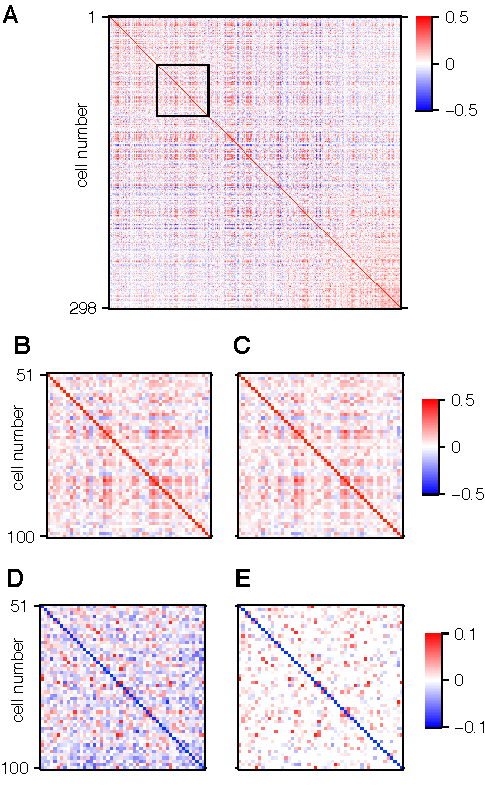
\includegraphics[width=8.3cm]{./figures/Figure01.pdf}
    \end{center}
    \caption{{\bf Illustration of regularized estimation of partial correlations.}
        {\bf A}. The sample correlation matrix of unprocessed somatic calcium signals from a population of cells in mouse visual cortex.
        The outlined square fragment is magnified in {\bf B}.
        {\bf C}. The same fragment of another estimate of the correlation matrix regularized to yield sparse partial correlations.
        Corresponding fragments of partial correlations matrices of the unregularized and regularized estimated are shown in {\bf D} and {\bf E}, respectively.
    }
    \label{fig:01}
\end{figure}

\begin{figure}[!ht]
    \begin{center}
        %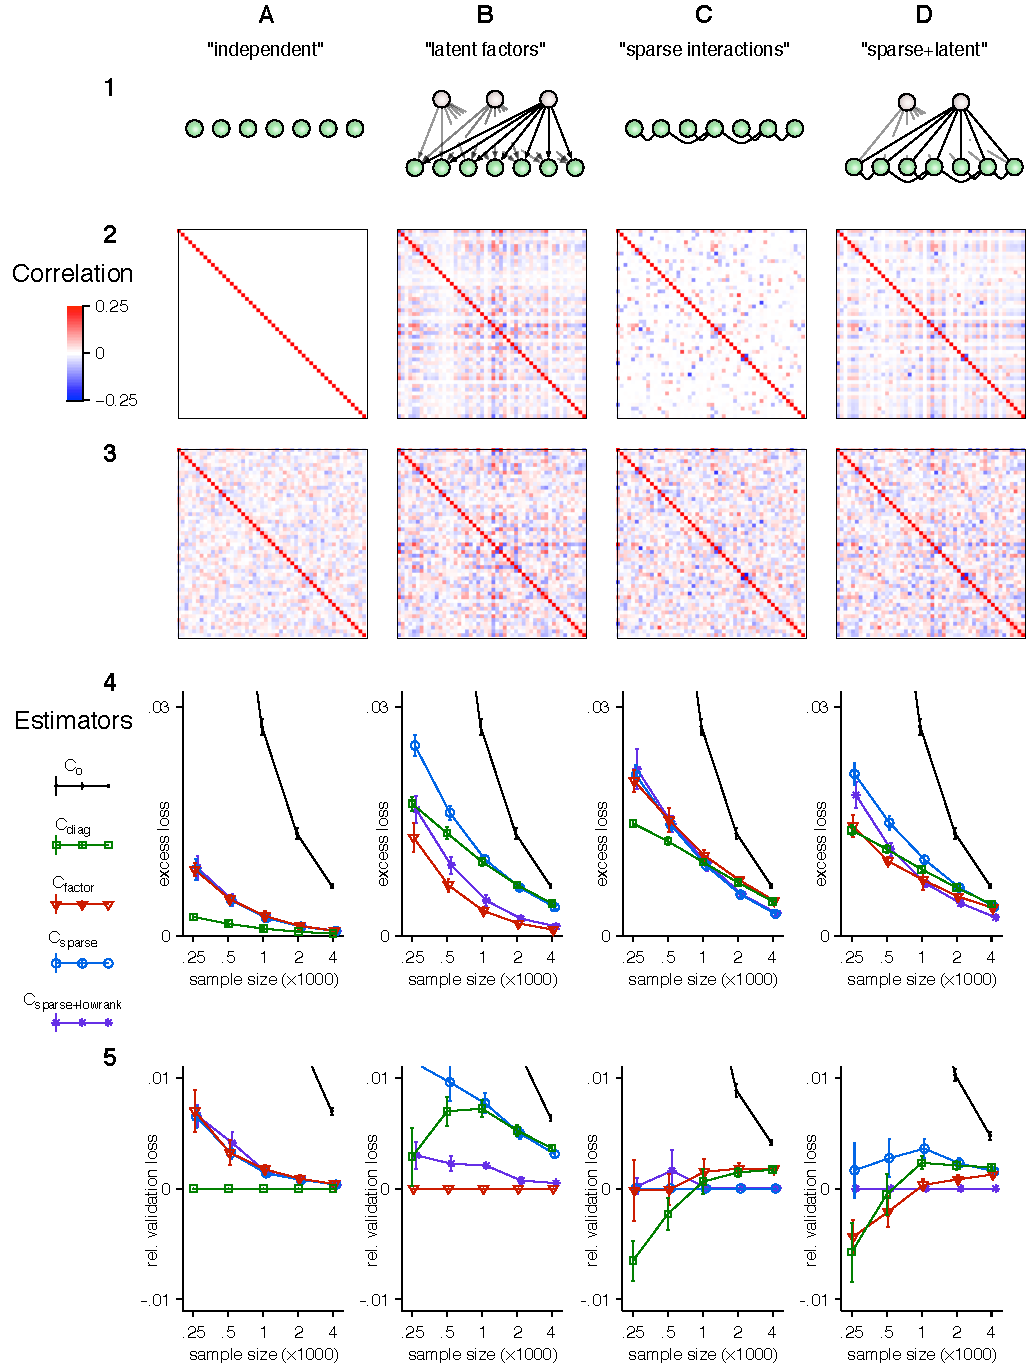
\includegraphics[width=17.35cm]{Figure02.pdf}
    \end{center}
    \caption{{\bf Estimators whose low-dimensional regularization targets can represent the structure of the true covariance matrix outperform other estimators.}
        {\bf Row 1.} Graphical representations of four types of low-dimensional structures of interactions between observed neurons (green spheres) and latent units (light-shaded spheres).
        In the `independent model' ({\bf A}), observed neurons exert no linear effects on one another neither directly nor through interactions with common latent units. 
        In `latent factors' ({\bf B}), the correlated activity of observed cells is driven by several latent units. 
        In `sparse interactions' ({\bf C}), the correlation matrix is defined by a set of linear interactions between observed neurons. 
        In `sparse+latent' ({\bf D}), correlations arise through direct linear interactions between some pairs of observed neurons and through interactions with common latent units. 
        {\bf Row 2.} Examples of $50\times 50$ correlation matrices corresponding to each type of low-dimensional structure. 
        The factor model ({\bf B}) has three latent units. 
        The partial correlation matrix of the sparse model ({\bf C}) is 73\% sparse.
        The `sparse+latent' matrix has one latent unit and its direct interactions are 78\% sparse.
        {\bf Row 3.} Examples of sample correlation matrices calculated from samples of 1000 observations taken from simulated random processes with corresponding correlation matrices from row 2.
        {\bf Row 4.} Average normalized Gaussian log-likelihood \emph{excess loss} (\ref{eq:excess-loss}) attained by each of the five estimators as a function of sample size. The error bars indicate the standard error of the mean based on 30 samples.
        {\bf Row 5.} Average normalized Gaussian log-likelihood \emph{validation loss} (\ref{eq:validation-loss}) attained by each of the five estimators. The values are relative to the validation loss of the estimator that matches the low-dimensional structure of the true covariance matrix. The error bars indicate the standard error of the mean based on 30 samples.
    }
    \label{fig:02}
\end{figure} 

\begin{figure}[!ht]
    \begin{center}
        %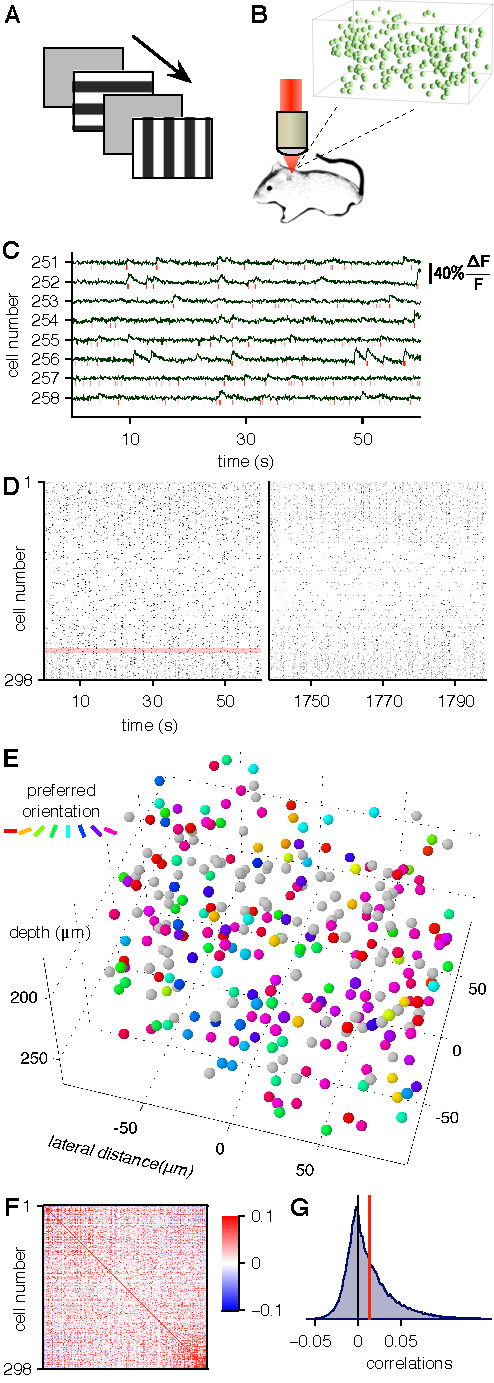
\includegraphics[width=8.3cm]{figures/Figure03.pdf}
    \end{center}
    \caption{{\bf Acquisition of neural signals for the estimation of noise correlations.}
    Visual stimuli comprising full-field drifting gratings interleaved with blank screens ({\bf A}) were presented to anesthetized mice while two-photon recordings of somatic calcium signals were collected using fast 3D random-access microscopy ({\bf B}). The visual stimulus included an initial period with 16 directions of motion for orientation tuning followed by a longer (15--20 min) period of stimulation with only 2 or 5 directions of motion for the computation of the noise correlation matrix. 
    {\bf C.} Representative calcium signals from eight cells out of 298 cells downsampled to 20 Hz. The inferred firing rate binned in 150 ms intervals are indicated by red ticks below each trace.
    {\bf D.} The raster plot of the inferred firing rates, binned in 150 ms intervals, from the entire population from the first (left) and last (right) minute of the entire recording.  The traces from {\bf C} are highlighted in red.
    {\bf E.} The spatial arrangement and orientation tuning of the 298 cells from the imaged site.
    {\bf F.} The noise correlation matrix of the activity of the neural population. 
    {\bf G.} The histogram of the noise correlation coefficients with the mean indicated by the red line.
}
    \label{fig:03}
\end{figure}

\begin{figure}[!ht]
    \begin{center}
        %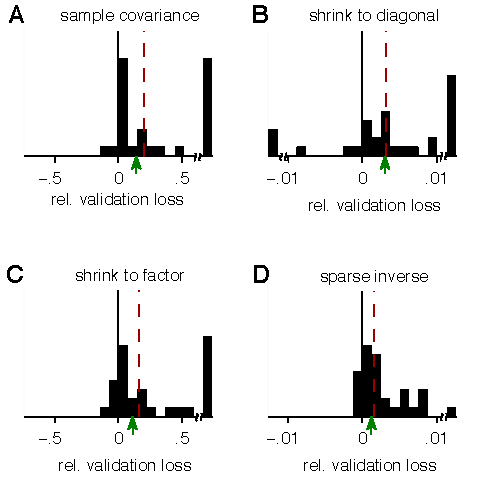
\includegraphics[width=8.3cm]{Figure04.pdf}
    \end{center}
    \caption{{\bf The sparse+lowrank estimator $C_{\sf sparse+lowrank}$ outperforms the other estimators on neural data.}
    {\bf A--D.} Histograms of average cross-validation loss differences of the respective estimators $C_0$, $C_{\sf diag}$, $C_{\sf factor}$, and $C_{\sf sparse}$ from $C_{\sf sparse+lowrank}$. 
    The histograms are based on 31 imaged sites in 24 mice. 
    All medians (red dashed lines) were significantly greater than zero, indicating the dominance of $C_{\sf sparse+lowrank}$ over the other estimators. 
    The green arrows indicate the results for the site shown in Fig.~\ref{fig:03} and Fig.~\ref{fig:05}
    }
    \label{fig:04}
\end{figure}
        
\begin{figure}[!ht]
    \begin{center}
        %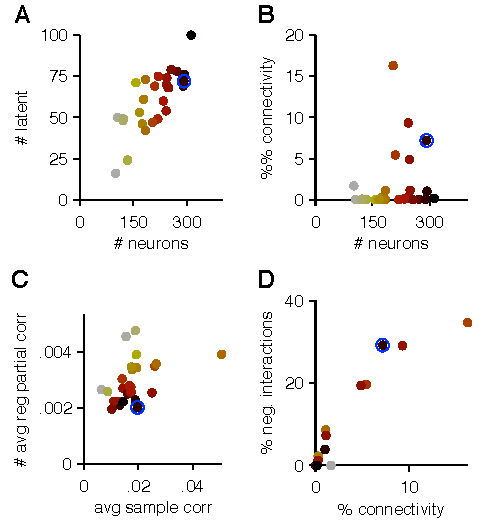
\includegraphics[width=17.35cm]{Figure05.pdf}
    \end{center}
    \caption{{\bf Example of low-dimensional correlation structure revealed by the sparse+low-rank estimator.}
    {\bf A.} The regularized estimate of the correlation matrix (top-right) closely approximates the sample correlation matrix (bottom left). 
    This close approximation is  also demonstrated by the scatter plot of the correlation coefficients produced by the two estimates ({\bf D}). 
    However, the partial correlation matrices from the two estimate show more pronounced differences ({\bf B} and {\bf E}). 
    {\bf C.} Furthermore, the partial correlation matrix of the regularized estimate is decomposed into a sparse component with 82.2\% off-diagonal zeros (bottom-left) and low-rank component of rank 15 (top-right).
    {\bf F.} The sparse component of the regularized partial correlation matrix had little resemblance to the sample correlations. The gray interval indicates the range of correlations containing 82.2\% of cells pairs, equal to the fraction of zeros in the sparse partial correlation matrix. This interval contained 58.9\% of the partial correlations. 
    {\bf G.} The graphical depiction of the positive (green) and negative (magenta) partial correlations as edges between observed neurons. The line density is proportional to the magnitude of the correlation.
    {\bf H.} A subset of neurons from the center of the cluster shown in {\bf G} showing the regularized partial correlations.
    {\bf I.} The same subset with sample correlations thresholded to match the sparsity of the regularized interactions.
}
\label{fig:05}
\end{figure}

\begin{figure}[!ht]
    \begin{center}
        %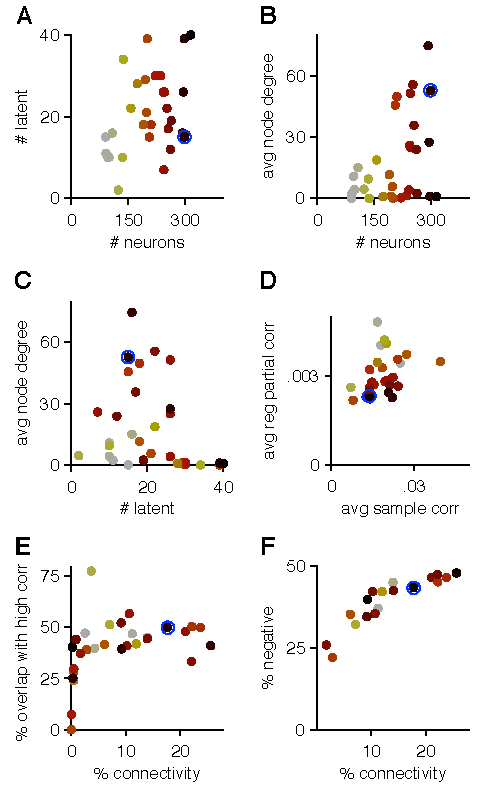
\includegraphics[width=17.35]{Figure06.pdf}
    \end{center}
    \caption{{\bf Properties of sparse+low-rank regularized estimates from all imaged sites}
    {\bf A.} The average sample correlations vs.~average partial correlations for each imaged site. In each plot, the red asterisk indicates the site shown in figures \ref{fig:03} and \ref{fig:05}.
    {\bf B.} The average node degree for sparse partial correlations vs.~population size in each imaged site. 
    {\bf C.} The number of inferred latent units vs.~population size in each imaged site.
    {\bf D.} The number latent units vs.~average node degree for sparse partial correlations for each site.
}
\label{fig:06}
\end{figure}

\begin{figure}[!ht]
    \begin{center}
        %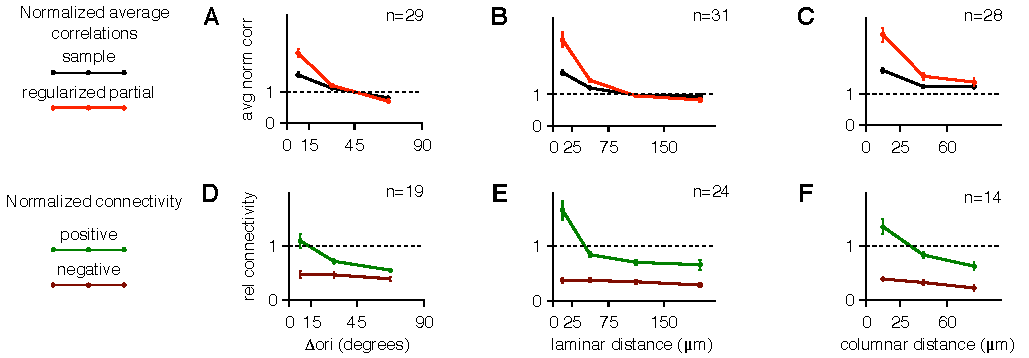
\includegraphics[width=17.35]{Figure07.pdf}
    \end{center}
    \caption{{\bf Dependence of correlations and partial correlations on orientation tuning differences and physical distance between cell pairs.}
    {\bf A--C.} Average sample correlations (black) and regularized partial correlations (red) between pairs of cells in the example site shown in previous figures. The correlations were normalized by the respective average correlations (\ref{fig:06}\,A).
    {\bf A.} Average correlations between pairs of neurons tuned to orientation with differences in preferred orientation in the intervals of 0--15$^\circ$, 15--45$^\circ$ and 45--90$^\circ$. 
    {\bf B.} Average correlations between pairs of neurons located at the same depth ($\pm$25$\mu$m) separated by lateral distances in the intervals of 0--25 $\mu$m, 25--75 $\mu$m, 75--150 $\mu$m, and 150+ $\mu$m.
    {\bf C.} Average correlations between pairs of neurons displaced laterally by less than 25 $\mu$m separated in depth by distances in the intervals of 0-25 $\mu$m, 25--60 $\mu$m, and 60+ $\mu$m.
    {\bf D--F.} Same measurements as {\bf A--D} averaged across multiple sites. Only sites that had at least 20 qualifying cell pairs in each of the intervals were included in the averages. The error bars indicate the standard error of the mean (often too small to be seen).
    {\bf G--I.} Normalized connectivity of positive (green) and negative (dark red) interactions from the sparse component of the regularized partial correlations in the example site show in previous figures. Normalized connectivity was computed as the fraction of pairs connected by interactions of corresponding signs in each interval divided by fraction of non-zero interactions across the entire site. The intervals are identical to those in {\bf A--C}.
    {\bf J--L.} Same measurements as in {\bf G--I} averaged across multiple sites. The error bars indicate the error of the mean. Only sites that had at least 20 qualifying pairs in each interval were included in the averages. 
}
\label{fig:07}
\end{figure}

\end{document}
